\clearpage
\section{Software}
\label{sec:software}
For this project, we needed quite a bit of software to be sure we could generate somewhat realistic workloads.
We also thought it important with predictability and put a lot of effort towards having a controlled environment. This goes for both the software and hardware involved.

Having done a bit of performance analysis before, we are aware of how difficult it can be to get meaningful and consistent results when analyzing programs and hardware interactions. We therefore decided to base ourselves on using some code we had written earlier in a information retrieval course. It is a simple search engine and indexer written in python, that does full text searches on a indexed corpus.

\subsection{Alternatives}
There are a few open source projects that are focused on information retrieval. We will here discuss some of the software we were considering using for this project.

\subsubsection{Lucene/Solr}
The most obvious software alternative might be the information retrieval system Lucene. Lucene is a heavier search engine written in Java, so it also requires a JVM to be running. The limited amount of less than 500MB of RAM was our main concern when we were discussing whether to use Lucene.

Additionally it is not a project and codebase we are familiar with.
This fact alone would make it hard for us to modify Lucene to our needs and be sure we got it right, and keep the level of control we wish for.

To make Lucene deployable in a distributed environment, a sideproject called Solr was started, and later included in the official Lucene project.
It offers a way to easily deploy Lucene and it's capabilities in a distributed manner, using among other things ZooKeeper for coordinating the cluster.

The concerns mentioned above and our unfamiliarity with the projects Lucene and Solr made us decide against using them.

\subsubsection{Sphinx}
Another open source project is the Sphinx search engine\cite{sphinx}. Sphinx provides full-text searching with a number of interfaces, including a SQL storage engine that can deliver results through a MariaDB server and connection. Spinx also has a query language much like SQL.

But this library also seems like overkill for our intents and purposes, so we decided against this.

\subsection{Setup}
As the authors had most experience with Arch Linux and it's environment, we decided to go with the distribution provided by the Arch Linux for ARM project.
The OS is distributed as a ISO image, which is written to the SD card using the UNIX disk utility {\tt dd}:
\begin{lstlisting}
dd if=inputimage.iso of=/dev/outdisk bs=1M
\end{lstlisting}

\subsection{Doing a search}
Since a significant part of our project is related to searching, we find it reasonable to include a section on how a search engine works in general.

Our engine consist of two parts: indexing and searching.
The search engine executes and scores a set of documents for given queries. For this work, it uses the dictionary, and a postings file.
The other part is the indexer, which builds an inverted index, the dictionary, and the postings file\cite{IntroIR} over a collection of documents (corpus).

When performing the indexing task, a loop runs over every document in the corpus.
For every word encountered in a document, the indexer emits a term, which is made into a token.
A token is what is left after post-processing a term. This processing usually includes stemming and removal of special characters.
The token is added to a dictionary and the document id is appended to the token's postings list. A counter is also kept along with the id to keep track of multiple occurrences of the same token in the same document.
The result of this loop is a dictionary of all unique tokens encountered, along with a postings list, naming all the documents that contain each token.

The dictionary contains the token, how many times it occurs in the collection, and a pointer to where this term is stored in the postings file.
The entries can be viewed as a tuple of the format:
$$<token, count, pointer>$$
The postings pointer is in our case an integer. This integer is the byte offset in the posting file where this terms posting list starts.

The postings entries are a list of tuples, in the format $$<docID, count>$$, giving the document id where the token occurred and the number of times it was seen in that document.

\begin{figure}[h]
    \center
    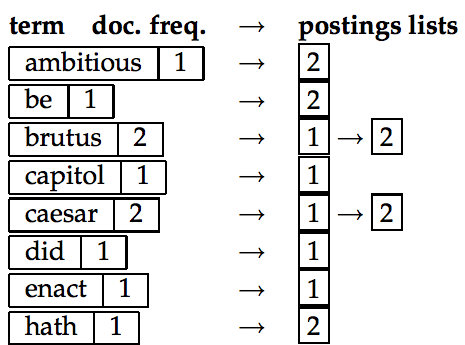
\includegraphics[width=0.5\textwidth]{software/index_postings_lists}
    \caption{A sample index and postings list. Credits goes to Introduction to IR\cite{IntroIR}.}
    \label{fig:index_postings_lists_sw}
\end{figure}

\subsection{Document scoring}
In the searching step one is usually working with a query containing one or more terms. For each token the corresponding postings list is fetched from disk (and cached). Each document is then scored according to a scoring scheme and a list of the documents sorted by the score is returned to the application.

To provide a rudimentary form of scoring, we have implemented the TF-IDF scoring system for queries. We are using the weighting scheme suggested by Introduction to Information Retrieval\cite{IntroIR}, {\tt lnc.ltc} in SMART notation\cite{tfidfsmart}.


\subsection{Operating system and environment}
Our operating system of choice is the Arch Linux for ARM project\cite{archarm}. This distribution provides us with a rolling release scheme, and eases development through the big and developer friendly package system AUR. If something is missing, it can be a lot easier to add it to all of the systems through the package manager.

The systems were mostly running on Linux kernel 3.6.11-18-ARCH, compiled for armv6l. This is as reported by running {\tt uname -a} on the target platform.

The systems also had the raspberrypi-firmware-tools packages, dated 20131021-1. Compilation was done with gcc:
\begin{lstlisting}[captionpos=b,caption={Output of {\tt gcc -v} and {\tt python --version}}]
$ gcc -v
Using built-in specs.
COLLECT_GCC=gcc
COLLECT_LTO_WRAPPER=/usr/lib/gcc/armv6l-unknown-linux-gnueabihf/4.7.2/lto-wrapper
Target: armv6l-unknown-linux-gnueabihf
Configured with: /build/src/gcc-4.7.2/configure --prefix=/usr --libdir=/usr/lib --libexecdir=/usr/lib --mandir=/usr/share/man --infodir=/usr/share/info --with-bugurl=https://bugs.archlinux.org/ --enable-languages=c,c++,fortran,lto,objc,obj-c++ --enable-shared --enable-threads=posix --with-system-zlib --enable-__cxa_atexit --disable-libunwind-exceptions --enable-clocale=gnu --disable-libstdcxx-pch --enable-libstdcxx-time --enable-gnu-unique-object --enable-linker-build-id --with-ppl --enable-cloog-backend=isl --disable-ppl-version-check --disable-cloog-version-check --enable-lto --enable-gold --enable-ld=default --enable-plugin --with-plugin-ld=ld.gold --with-linker-hash-style=gnu --disable-multilib --disable-libssp --disable-build-with-cxx --disable-build-poststage1-with-cxx --enable-checking=release --host=armv6l-unknown-linux-gnueabihf --build=armv6l-unknown-linux-gnueabihf --with-arch=armv6 --with-float=hard --with-fpu=vfp
Thread model: posix
gcc version 4.7.2 (GCC)

$ python --version
Python 2.7.5
\end{lstlisting}

\subsection{Booting and deployment}
To collaborate and distribute our code, we use a git repository stored at GitHub\cite{github}. We also agreed upon a set folder structure to make it easier to maintain and deploy our code, storing the git directory under {\tt /home/<user>/src/project}.
The username is the same for all nodes.

We created a systemd script that runs at boot, which does a repository pull and builds all the code, then run it. So to deploy a new update, we would cut the power to the rig and start it again.
This proved very efficient in practice and saved us a lot of manual work, like manually logging in and updating each individual system. The boot script is given in listing \ref{lst:bootscript}.
\begin{lstlisting}[captionpos=b,caption={Our Systemd boot script. It launches a script that makes sure datetime is set before launching the update script.},label={lst:bootscript}]
#-/etc/systemd/system/pinode.service
[Unit]
Description=PI search service
ConditionPathExists=/etc/rc.local

[Service]
Type=forking
ExecStart=/etc/rc.local
TimeoutSec=0
StandardOutput=tty
RemainAfterExit=yes
SysVStartPriority=99

[Install]
WantedBy=multi-user.target

#-/etc/rc.local
su king -c "/home/king/src/project/boot_pinode.py"

#-boot_pinode.py
projectdir = "/home/king/src/project"
hostname = socket.gethostname()

os.chdir(projectdir)

def update_git():
    subprocess.call(["git", "pull"])
    subprocess.call(["make"])

def launch_load_distr():
    subprocess.call(["bin/load_distributor_bin"])

def launch_search_engine():
    subprocess.call(["bin/search_bin"])

while True:
    update_git()

    if hostname[len(hostname)-1] == '0':
        launch_load_distr()
    else:
        launch_search_engine()

\end{lstlisting}

\subsection{Load generator}
The purpose of the load generator is to generate pseudo-random queries and send these to the load distributor to simulate load on the cluster. These queries are of varying length and contains tokens found in the dictionary.

The load generator runs on several threads, where one thread is responsible for receiving answers for the queries, and one or more threads are responsible for generating load for the system. The load generator is implemented in python and meant to be run on a node outside the cluster.

The load generator includes some configurable parameters, most importantly the frequency of the queries being sent and the number of threads sending queries simultaneously.

The load generator was later edited to also be able to send queries directly to the workers and by bypassing the load distributor all together. This simulates moving the load distribution out to the client application. In this case, we have one thread for each worker that sends queries at a given interval.

\subsection{Load distribution}
One of the nodes in the cluster will be in charge of load distribution. The load distributor node will receive all the queries and then forward them to the worker nodes.
The node employs the very simple load balancing scheme of $$rand() \bmod N,$$ where N is the number of nodes in the cluster.
The messages from the load distributor to the worker nodes includes information of where to deliver the search results when they are ready.
This scheme is simple, but could also prove to be a bottleneck of the system. Seeing as all communication has to go through this node we could end up with the performance of the cluster being limited by the load distributor.

\subsection{Original search engine - python version}
The python version we were basing our program on, relied heavily upon the python library Natural Language Toolkit\cite{nltk} (NLTK).
NLTK provides a lot of useful methods for processing natural languages in Python, including different tools for stemming and other tokenization tricks.
Stemming is the process of reducing inflected or conjugated words into their basic or root form. Examples include removal of prefixes, suffixes, tense and vowel changes. I.e. words like ``fishing'', ``fisher'' and ``fished'' all end up mapping to the same stem ``fish''.

The toolkit also provides stop word lists (words like {\em and}, {\em or}, {\em on}, {\em the} and so on) and improved splicing of natural language sentences into token.
NLTK however only exist for python, so if we were to write a C version, we would have to port the library, or at least the functionality we use.
As this is a lot of work to implement, and well beyond the scope of our work here, we have chosen to do the indexing in python and deliver and calculate search results based only on the stemmed forms for the C program.

The indexing is a very slow operation. It is however done very rarely, and only when incorporating new documents (new corpus) into the search results. This operation is in our case not even time critical, so we think it is a fair simplification to leave this job for a faster computer that can run python.

\subsection{Optimized C-port}
In practice we experienced serious performance issues with our python code, often showing response times in the hundreds of milliseconds on the cluster. We therefore decided to rewrite the search program using C. This proved it both challenging and useful to control what exactly is present in memory at every moment, in addition to the extra work of having to control memory allocation.

Our current implementation caches everything it looks up in memory. We did not have the time to write a proper system for managing the amount of memory consumed by the cache.
This could lead to out of memory issues, but the internal structures will be within bounds of the size of the postings file, which is by far the most dominant element with regards to memory usage.
The reader should note that as a consequence, we have to keep an eye on the size of the postings file, so as not to let the nodes run out of memory and crash. We did not run into any problems with this approach in practice, as our corpus is fairly small.

The program reads the dictionary structure into memory on startup. It provides O(1) lookup on query terms in a hash map, using the library {\tt uthash}\cite{uthash}.

\begin{lstlisting}[style=customc,captionpos=b,caption={Structure of a dictionary entry (term)},numbers=left]
typedef struct {
    char* term;
    uint32_t byte_offset;
    uint32_t occurences;
    postings_entry* posting;
    UT_hash_handle hhd;         /* makes this structure hashable */
} dictionary_entry;
\end{lstlisting}
\subsubsection{uthash}
{\tt uthash} is a small library with a set of convenient preprocessor macros for creating and managing hash tables in C.
{\tt uthash} does constant time $$O(1)$$ lookups, inserts and deletes, and comes with a number of different hash functions in case your key domain is not well suited for the default hash function.
{\tt uthash} can hash strings, integers, pointers and the bytes in a structure a pointer points to.

\subsubsection{Experiences}
The first testings of the C-port showed significant improvements in delivery speed.
It further confirmed that managing memory yourself is desirable for performance, and is especially important in an environment where resources are scarce.
When blasting the searching code with queries, we quickly maxed out the available memory.
These memory leaks were later fixed, and the program now experiences constant memory usage.

The difference in developing platform, with x86\_64 Darwin compared to the ARMv6 runtime environment did not impose any extra difficulties, except for a single case of some odd pointer behavior.
The rest of the time, the code behaved as expected from one platform to the other, for both Python and C.

For comparison between the two languages, we created a test set of 100,000 queries. We then ran this test set against the reference MacBook computer, and on the Pi, both for Python and {C}.
The results are given in Table \ref{tbl:runtimes_ports}.

For the relatively quick {Core i5}, the python code need 10 times longer to run the queries than the C code. This difference in performance seem reasonable compared to known sources.
The Python code is however detrimental to the performance for the weaker Pi. The same 100,000 queries takes 84 seconds to run in C, but takes 24 times longer in python.

\begin{table}[h]
	\begin{center}
	\begin{tabular}{|r|r|r|r|}
	\hline
	   & \multicolumn{1}{|c|}{MacBook} & \multicolumn{1}{|c|}{PI (OC)}  & \multicolumn{1}{|c|}{PI} \\
	\hline
	C      & 4.78 & 55.93 & 84.75     \\
	\hline
	Python & 49.41 & FIND & 2046.77   \\

	\hline
	\end{tabular}
	\caption{Runtime (in seconds) for C and Python code on 100,000 queries. OC is the overclocked Pi.}
	\label{tbl:runtimes_ports}
	\end{center}
\end{table}
